	\chapter{}
\label{lecture12}
\section{Уравнение малых колебаний струны (продолжение).}
\label{lecture12section1}
Возвращаемся к выведенному нами уравнению колебаний струны
\begin{equation}
	\label{l12:eq:1}
	\hfill\pder{}{x}\big(\mu\cdot u_x\big)-\pder{}{t}\big(\rho\cdot u_t\big)+f(x,t)=0.\hfill
\end{equation}
Пусть начальное положение и начальная скорость струны задаются равенствами 
\begin{equation}
	\label{l12:eq:2}
	\hfill u(x,0)=\phi(x),\quad u_t(x,0)=\psi(x),\hfill
\end{equation} 
где $\phi(x)$ и $\psi(x)$ --- известные функции. Граничные условия возьмём простейшие --- предположим, что концы струны закреплены.
\begin{equation}
	\label{l12:eq:3}
	\hfill u(a,t)=0,\quad u(b,t)=0.\hfill
\end{equation}

При постановке задач, приводящих к уравнениям в частных производных (так же как в задачах, связанных с обыкновенными дифференциальными уравнениями) огромное значение имеет \emph{корректность постановки задачи}.
\begin{_def}
	Мы говорим, что \textbf{задача поставлена корректно}, если для рассматриваемого уравнения решение:
	\begin{enumerateD}
		\item существует;
		\item единственно;
		\item непрерывно зависит от входных данных.
	\end{enumerateD} 
\end{_def}
\noindent Поясним сказанное в основном применительно к задаче~\eqref{l12:eq:1}--\eqref{l12:eq:3}.
\begin{enumerateD}
	\item На практике существование решения большей частью доказывается прямым его построением. Но решение может не существовать, если наложить избыточные требования. Приведём два примера.
	\begin{enumerateD}
		\item Пусть решение уравнения~\eqref{l12:eq:1} ищется в классе $\Cfn{2}(\overline{\Omega})$, но мы кроме начальных условий~\eqref{l12:eq:2} задаём дополнительно начальное ускорение $u_{tt}(x,0)=h(x)$. Но из уравнения~\eqref{l12:eq:1}
		\begin{equation*}
			u_{tt}=\left(\pder{}{x}\big(\mu\cdot u_x\big)-\rho_t\cdot u_t+f\right)\Biggm/\rho,\quad t\geqslant0.
		\end{equation*}
		Откуда при $t=0$ в силу условий~\eqref{l12:eq:2}
		\begin{equation}
			\label{l12:eq:4}
			u_{tt}(x,0)=\left(\mu_x\cdot\phi_x+\mu\cdot\phi_{xx}-\rho_t\cdot\psi+f\right)\bigm/\rho,
		\end{equation}
		где правая часть полностью определяется условиями~\eqref{l12:eq:2}. Поэтому если функция $h(x)$ не равна правой части~\eqref{l12:eq:4}, то решение задачи~\eqref{l12:eq:1}--\eqref{l12:eq:3} с условием $u_{tt}(x,0)=h(x)$ не существует.
		
		\item Пусть решение ищется в классе $\Cfn{2}(\Omega)$, $\rho(x,t)\in\Cfn{1}(\Omega)$, $\mu(x,t)\in\Cfn{1}(\Omega)$, а функция $f(x,t)$ разрывна на некоторой кривой $\Gamma\subset\Omega$. Ясно, что равенство~\eqref{l12:eq:1} на $\Gamma$ не выполняется. 
	\end{enumerateD}
	\item О единственности. Решение может быть не единственно, если заданных условий не достаточно для выделения одного решения из класса всех решений задачи~\eqref{l12:eq:1}--\eqref{l12:eq:3}. Например, мы увидим, что если задать только $u(x,0)$ или только $u_t(x,0)$, то решение задачи~\eqref{l12:eq:1}--\eqref{l12:eq:3} не единственно. Ситуация аналогична положению в обыкновенных дифференциальных уравнениях. Например, для уравнения 
	\begin{equation*}
		\hfill \dder{y}{t}=R(t,y,y')\hfill
	\end{equation*}
	решение не единственно на отрезке $[t_0,t_1]$, если мы задали только $y(t_0)$ или только $y'(t_0)$.
	Что касается единственности решения задачи~\eqref{l12:eq:1}--\eqref{l12:eq:3}, то она будет доказана ниже для различных типов граничных условий.
	\item Непрерывная зависимость от входных данных. В рассматриваемой ситуации --- это непрерывная зависимость от начальных условий $\phi(x)$ и $\psi(x)$. Непрерывная зависимость означает, что малым изменениям $\phi(x)$ и $\psi(x)$ должно отвечать малое изменение решения. Дадим точное определение. 
	\begin{_def}
		Пусть $\phi$, $\psi$ и $\widehat{\phi}$, $\widehat{\vphantom{\phi}\smash{\!\psi}}$ некоторые начальные условия для уравнения \eqref{l12:eq:1} и $u$ и $\widehat{u}$ --- отвечающие им решения. Будем говорить, что для решения задачи~\eqref{l12:eq:1}--\eqref{l12:eq:3} имеет место непрерывная зависимость от начальных данных, если по $\forall\eps>0$, $T>0$ можно найти $\delta>0$ так, что при 
		\begin{gather*}
			\big|\phi(x)-\widehat{\phi}(x)\big|<\delta,\ \big|\psi(x)-\widehat{\vphantom{\phi}\smash{\!\psi}}(x)\big|<\delta\quad\forall x\in[a,b],
			\intertext{выполняется}
			\big|u(x,t)-\widehat{u}(x,t)\big|<\eps,\quad\forall x\in[a,b],\ t\in[0,T].
		\end{gather*} 
	\end{_def}
	\noindent Мы докажем непрерывную зависимость решений задачи~\eqref{l12:eq:1}--\eqref{l12:eq:3} от начальных условий при постоянных $\rho$ и $\mu$ позднее. 
\end{enumerateD}

А сейчас докажем единственность решения задачи~\eqref{l12:eq:1}--\eqref{l12:eq:3} при $\rho=\rho(x)$ (нет зависимости от времени) в случае граничных условий~\eqref{l12:eq:3a} или~\eqref{l12:eq:3b}
\addtocounter{equation}{-2} 
\begin{subequations}
	\begin{gather}
		u(a,t)=h_1(t),\quad u(b,t)=h_2(t)\label{l12:eq:3a}\\
		\hfill u_x(a,t)=g_1(t),\quad u_x(b,t)=g_2(t),\label{l12:eq:3b}
	\end{gather}
\end{subequations}	
\addtocounter{equation}{1}где $h_i(t)$, $g_i(t)$, $i=1,2$ --- заданные функции.

Пусть $u_1$ и $u_2$ --- два решения задачи~\eqref{l12:eq:1},~\eqref{l12:eq:2},~\eqref{l12:eq:3a} или~\eqref{l12:eq:1},~\eqref{l12:eq:2},~\eqref{l12:eq:3b}. Положим $u\eqdef u_1-u_2$. Тогда функция $u(x,t)$ удовлетворяет уравнению 
\begin{equation}
	\label{l12:eq:5}
	\hfill\pder{}{x}\big(\mu\cdot u_x\big)-\rho(x)\cdot\pder{^2 u}{t^2}=0\hfill
\end{equation} 
с нулевыми начальными и граничными условиями 
\begin{equation}
	\label{l12:eq:6}
	u(x,0)=u_t(x,0)=0,
\end{equation}
и
\begin{subequations}
	\begin{gather}
		u(a,t)=u(b,t)=0\hfill\label{l12:eq:7a}
		\intertext{или}
		u_x(a,t)=u_x(b,t)=0.\label{l12:eq:7b}
	\end{gather}
\end{subequations}
\newpage

Составим интеграл энергии $E(t)$ в момент $t$. Согласно предыдущему 
\begin{equation*}
	\hfill E(t)=\int\limits_a^b\left(\frac{\rho\cdot u^2_t}{2}+\frac{\mu\cdot u^2_x}{2}\right)\,dx.\hfill
\end{equation*} 
Покажем, что $E(t)$ не зависит от $t$. Тогда 
\begin{equation}
	\label{l12:eq:8}
	\hfill E(t)=E(0),\quad t\geqslant0,\hfill
\end{equation}
но в силу \eqref{l12:eq:6} $E(0)=0$ и значит $E(t)\equiv0$ при $\forall t$. Но это возможно лишь при $u_x\equiv0$, $u_t\equiv0$, то есть при $u=const$. Отсюда очевидно, в силу~\eqref{l12:eq:6} $u\equiv0$, то есть единственность доказана. Остаётся установить~\eqref{l12:eq:8}. Для этого найдём $\der{E}{t}$. Имеем 
\begin{equation*}
	\der{E}{t}=\int\limits_a^b\left(\rho\cdot u_t\cdot u_{tt}+\mu\cdot u_x\cdot u_{xt}\right)\,dx=\int\limits_a^b\left[\rho\cdot u_t\cdot u_{tt}-\pder{}{x}\big(\mu\cdot u_x\big)\cdot u_t\right]\,dx+\mu\cdot u_x\cdot u_t{\mathop{\Big|}\limits_a^b}\phantom{|}{\vphantom{\bigg|}}^{\footnotemark{}}_{\displaystyle.}
\end{equation*}
\footnotetext{Мы интегрировали по частям слагаемое $\big(\mu\cdot u_x\big)\cdot u_{xt}$.}
При условии~\eqref{l12:eq:7a} $u_t(a,t)=u_t(b,t)=0$. При условии~\eqref{l12:eq:7b} $u_x(a,t)=u_x(b,t)=0$. Поэтому внеинтегральный член в формуле для $\displaystyle\der{E}{t}$ равен нулю, а интеграл равен нулю вследствие~\eqref{l12:eq:5}. Следовательно $\displaystyle\der{E}{t}\equiv0$ и~\eqref{l12:eq:8} --- доказано. Таким образом единственность решения задач~\eqref{l12:eq:1},~\eqref{l12:eq:2},~\eqref{l12:eq:3a} и~~\eqref{l12:eq:1},~\eqref{l12:eq:2},~\eqref{l12:eq:3b} доказана.
\vspace{0.2cm}

\noindent\textbf{Задание. }Рассмотреть случай упругого закрепления (в интеграле энергии появятся дополнительные члены).

\section{Свободные колебания однородной струны.}
\label{lecture12section2}
Пусть струна однородна, то есть $\rho$ и $\mu$ --- константы. Поделим обе части уравнения~\eqref{l12:eq:1} на $\rho$ и положим, $a^2\eqdef{\mu}\bigm/{\rho}$. Тогда уравнение~\eqref{l12:eq:1} можно записать в виде
\begin{equation}
	\label{l12:eq:9}
	\hfill u_{tt}=a^2\cdot u_{xx}+f(x,t)\bigm/\rho\hfill
\end{equation}
Мы рассматриваем свободные колебания струны и значит $f(x,t)=0$. Однако уместно заметить, что если бы на струну действовала распределённая сила с плотностью $f(x,t)$ на единицу длины, то в уравнение колебаний вошла бы --- как видно из~\eqref{l12:eq:9} --- плотность силы на единицу массы, то есть $f\bigm/\rho$.

Будем считать, что струна в невозмущённом состоянии занимает отрезок $[0,l]$ оси $x$. Этого можно добиться, если положить $x'=x-a$ и тогда $x'\in[0,l]$, где $l=b-a$. Разумеется <<штрих>> у $x'$ далее опускаем.
\begin{gather}
	\intertext{Итак, будем решать уравнение}
	\label{l12:eq:10}u_{tt}=a^2\cdot u_{xx}
	\intertext{с начальными условиями}
	\label{l12:eq:11}u(x,0)=\phi(x),\ u_t(x,0)=\psi(x)\quad x\in[0,l]
	\intertext{и простейшими граничными условиями}
	\label{l12:eq:12}u(0,t)=0,\ u(l,t)=0
\end{gather}
Решение задачи~\eqref{l12:eq:10}--\eqref{l12:eq:12} будем искать методом Фурье (он же --- метод разделения переменных, он же --- метод суперпозиции стоячих волн).

Сначала попытаемся найти частное решение $u_{\text{ч}}(x,t)$ задачи~\eqref{l12:eq:10}, \eqref{l12:eq:12} (то есть без учёта начальных условий). Это решение будем искать в виде 
\begin{equation*}
	\hfill u_{\text{ч}}(x,t)=X(x)\cdot T(t),\hfill
\end{equation*} 
где $X(x)$, $T(t)$ --- неизвестные функции, зависящие каждая соответственно только от $x$ и $t$. Подставим $u_{\text{ч}}(x,t)$ в~\eqref{l12:eq:10}. Получим
\begin{equation*}
	\hfill	T''\cdot X=a^2\cdot X''\cdot T,\hfill
\end{equation*} 
где штрихи означают производные по аргументам. Поделив обе части этого равенства на произведение $a^2\cdot X\cdot T$ получим 
\begin{equation}
	\label{l12:eq:13}
	\hfill\frac{T''}{a^2\cdot T}=\frac{X''}{X}.\hfill
\end{equation}
Так как левая часть~\eqref{l12:eq:13} не зависит от $x$, то и правая тоже. Так как правая часть~\eqref{l12:eq:13} не зависит от $t$, то и левая тоже. Поэтому отношение в~\eqref{l12:eq:13} равно константе, которую мы обозначим через ($-\lambda$), то есть
\begin{gather}
	\frac{T''}{a^2\cdot T}=-\lambda,\ \frac{X''}{X}=-\lambda,\notag
	\intertext{откуда}
	T''+a^2\cdot\lambda\cdot T=0\label{l12:eq:14}\\
	-X''=\lambda\cdot X\label{l12:eq:15}.	
\end{gather} 
Из~\eqref{l12:eq:12} следует, что 
\begin{gather}
	T(t)\cdot X(0)=0,\ T(t)\cdot X(l)=0,\quad\forall t \notag
	\intertext{и поэтому}
	X(0)=0,\ X(l)=0\label{l12:eq:16}
\end{gather}
Таким образом число $\lambda$ и функция $X(x)$ есть собственное значение и отвечающая ему собственная функция оператора Штурма $\left(-\dder{}{x}\right)$ с граничными условиями~\eqref{l12:eq:16}. Мы знаем, что 
\begin{equation*}
	\hfill\lambda_k=\left(\frac{\pi\cdot k}{l}\right)^2,\ X_k=\sqrt{\frac{2}{l}}\cdot\sin\left(\frac{\pi\cdot k}{l}\cdot x\right),\quad k=1,2,\ldots\hfill
\end{equation*}
Далее подставим в~\eqref{l12:eq:14} $\lambda=\lambda_k$ и положим $\omega^2_k\eqdef a^2\cdot\lambda_k$. Тогда из~\eqref{l12:eq:14} получим, что 
\begin{equation*}
	\hfill T(t)=T_k(t)=A_k\cdot\cos(\omega_k\cdot t)+B_k\cdot\sin(\omega_k\cdot t),\hfill
\end{equation*}
где $A_k$ и $B_k$ --- произвольные константы. 

Таким образом искомое решение $u_{\text{ч}}(x,t)$ есть $u_k(x,t)=X_k(x)\cdot T_k(t)$. $u_k(x,t)$ есть решение задачи~\eqref{l12:eq:10},~\eqref{l12:eq:12}. Конечная сумма 
\begin{equation*}
	\hfill S_n(x,t)=\sum\limits_{k=1}^n u_k(x,t)\hfill 
\end{equation*}
тоже есть решение задачи~\eqref{l12:eq:10},~\eqref{l12:eq:12}. А теперь рассмотрим бесконечную сумму 
\begin{equation*}
	\hfill u\eqdef\sum\limits_{k=1}^{\infty}u_k(x,t)\hfill
\end{equation*}
и будем считать, что коэффициенты $A_k$, $B_k$ в формуле $T_k(t)$ выбраны так, что ряд $\sum\limits_{k=1}^{\infty}u_k(x,t)$ сходится равномерно и допускает почленное дифференцирование два раза по $x$ и по $t$. Тогда подставляя этот ряд в уравнение~\eqref{l12:eq:10} и в граничные условия~\eqref{l12:eq:12} убеждаемся, что функция $u=\sum\limits_{k=1}^{\infty}u_k(x,t)$ удовлетворяет и~\eqref{l12:eq:10}, и~\eqref{l12:eq:12}. Попробуем теперь найти пока <<свободные>> константы $A_k$ и $B_k$ так, чтобы функция $u$ удовлетворяла начальным условиям~\eqref{l12:eq:11}
\begin{equation}
	\label{l12:eq:17}
	\hfill u(x,0)=\sum\limits_{k=1}^{\infty}u_k(x,0)=\sum\limits_{k=1}^{\infty}A_k\cdot X_k(x)=\phi(x)\hfill
\end{equation}
\begin{equation}
	\label{l12:eq:18}
	\hfill u_t(x,0)=\sum\limits_{k=1}^{\infty}\pder{u_k}{t}(x,0)=\sum\limits_{k=1}^{\infty}B_k\cdot\omega_k\cdot X_k(x)=\psi(x)\hfill
\end{equation}
Равенства~\eqref{l12:eq:17} и~\eqref{l12:eq:18} --- это разложение функций $\phi(x)$ и $\psi(x)$ по собственным функциям оператора Штурма. По теореме Стеклова такое разложение возможно, а характер сходимости зависит от свойств функций $\phi(x)$ и $\psi(x)$. Из~\eqref{l12:eq:17} и~\eqref{l12:eq:18} имеем 
\begin{equation*}
	\hfill A_k=\big(\phi,X_k\big)=\int\limits_0^l\phi(\xi)\cdot X_k(\xi)\,d\xi,\hfill
\end{equation*}
\begin{equation*}
	\hfill B_k=\frac{\big(\psi,X_k\big)}{\omega_k}=\frac{1}{\omega_k}\cdot\int\limits_0^l\psi(\xi)\cdot X_k(\xi)\,d\xi,\hfill
\end{equation*}
где $\displaystyle\omega_k=a\cdot\sqrt{\lambda_k}=a\cdot\frac{\pi\cdot k}{l}$, $\displaystyle  X_k(\xi)=\sqrt{\frac{2}{l}}\cdot\sin\left(\frac{\pi\cdot k}{l}\cdot\xi\right)$.

Таким образом, если найденные коэффициенты $A_k$, $B_k$ обеспечивают равномерную сходимость ряда $\sum\limits_{k=1}^{\infty}u_k$ и возможность его двукратного почленного дифференцирования по $x$ и по $t$, то функция $u=\sum\limits_{k=1}^{\infty}u_k(x,t)$ есть решение задачи~\eqref{l12:eq:10}--\eqref{l12:eq:12}. 

Достаточным условием этого являются следующие требования к функциям $\phi(x)$ и $\psi(x)$:
\begin{gather}
	\label{l12:eq:ast}
	\begin{cases}
		\phi\in\Cfn[{[0,l]}]{2},\ \psi\in\Cfn[{[0,l]}]{1},\ \phi'''\text{ и }\psi''\text{ --- кусочно непрерывны}\\
		\phi(0)=\phi(l)=0,\ \phi''(0)=\phi''(l)=0,\ \psi(0)=\psi(l)=0 
	\end{cases}\tag{$*$}
\end{gather}
\vspace{0,2cm}

\noindent\textbf{Задание. }Докажите, что условия~\eqref{l12:eq:ast} действительно обеспечивают требуемые свойства ряда $\sum\limits_{k=1}^{\infty}u_k(x,t)$ (используйте интегрирование по частям для оценок $A_k$ и $B_k$).

\begin{_rem}
	Условия~\eqref{l12:eq:ast} являются достаточными для применимости метода разделения переменных. Однако метод характеристик, с которым вы познакомитесь несколько позже, позволяет построить решение задачи~\eqref{l12:eq:10}--\eqref{l12:eq:12} при более слабых, чем~\eqref{l12:eq:ast}, ограничениях на функции $\phi(x)$ и $\psi(x)$.   
\end{_rem}

Вернёмся к построенному нами решению $u=\sum\limits_{k=1}^{\infty}u_k$ и запишем функцию $u_k$ в изменённом виде:
\begin{gather*}
	u_k(x,t)=X_k(x)\cdot\big(A_k\cdot\cos(\omega_k\cdot t)+B_k\cdot\sin(\omega_k\cdot t)\big)=C_k\cdot\sin(\omega_k\cdot t+\beta_k)\cdot X_k(x),
	\intertext{где}
	C_k=\sqrt{A^2_k+B^2_k},\text{ а угол } \beta_k\text{ определяется из соотношений }\sin\beta_k=A_k\!\bigm/\!C_k,\ \cos\beta_k=B_k\!\bigm/\!C_k. 
\end{gather*}
Функция $u_k$ называется \emph{стоячей волной} (отсюда одно из названий метода --- метод суперпозиции стоячих волн). Каждая точка $x_0$ стоячей волны $u_k$ колеблется с частотой $\omega_k$ и амплитудой \\$C_k\cdot X_k(x_0)$. Те точки волны $u_k(x,t)$, для которых амплитуда равна нулю для всех $t$, называются её узлами. Профиль стоячей волны определяется функцией $X_k(x)$; в данном случае это синусоида. Частота $\omega_k=\lambda_k\cdot\sqrt{{\mu}\!\bigm/\!{\rho}}$ стоячей волны обратно пропорциональна корню из плотности струны и прямо пропорциональна корню из жёсткости струны, что качественно естественно из физических соображений. 

\section{Понятие о функции Грина.}
\label{lecture12section3}
Если в выражение $u_k(x,t)$ подставить найденные значения коэффициентов $A_k$ и  $B_k$, то мы получим
\begin{equation}
	\label{l12:eq:19}
	u(x,t)=\sum\limits_{k=1}^{\infty}\int\limits_0^l\frac{1}{\omega_k}\cdot\sin(\omega_k\cdot t)\cdot X_k(x)\cdot X_k(\xi)\cdot\psi(\xi)\,d\xi+ \sum\limits_{k=1}^{\infty}\int\limits_0^l\cos(\omega_k\cdot t)\cdot X_k(x)\cdot X_k(\xi)\cdot\phi(\xi)\,d\xi.
\end{equation}
Введём в рассмотрение функцию
\begin{equation}
	\label{l12:eq:20}
	 G(x,\xi,t)=\sum\limits_{k=1}^{\infty}\frac{1}{\omega_k}\cdot\sin(\omega_k\cdot t)\cdot X_k(x)\cdot X_k(\xi),
\end{equation}
которая называется функцией Грина для задачи~\eqref{l12:eq:10}--\eqref{l12:eq:12}. Так как частоты $\omega_k$ растут со скоростью $k$, то ряд для функции $G(x,\xi,t)$ сходится в среднем по $\xi$ при любых фиксированных $x$ и $t$ (докажем позже). Поэтому первую сумму в~\eqref{l12:eq:19} можно записать в виде 
\begin{equation*}
	\hfill\int\limits_0^l G(x,\xi,t)\cdot\psi(\xi)\,d\xi.\hfill
\end{equation*}
Что касается второй суммы в~\eqref{l12:eq:19} то формально её можно записать в виде 
\begin{equation*}
	\hfill\int\limits_0^l G_t(x,\xi,t)\cdot\phi(\xi)\,d\xi,\hfill
\end{equation*}
хотя, конечно, ни о каком почленном дифференцировании ряда для $G(x,\xi,t)$ речи быть не может: полученный ряд расходится. Поэтому выражение $\int\limits_0^l G_t(x,\xi,t)\cdot\phi(\xi)\,d\xi$ надо понимать как предел 
\begin{equation*}
	\hfill\lim\limits_{n\to\infty}\int\limits_0^l\pder{S_n}{t}(x,\xi,t)\cdot\phi(\xi)\,d\xi,\hfill
\end{equation*}
где $S_n(x,\xi,t)=\sum\limits_{k=1}^n\sin\big(\omega_k\cdot t\big)\cdot X_k(x)\cdot X_k(\xi)\bigm/\omega_k$ --- частная сумма ряда~\eqref{l12:eq:20}. С учётом сказанного мы можем записать равенство~\eqref{l12:eq:19} в виде
\begin{equation}
	\label{l12:eq:21}
	\hfill u(x,t)=\int\limits_0^l G(x,\xi,t)\cdot\psi(\xi)\,d\xi+\int\limits_0^l G_t(x,\xi,t)\cdot\phi(\xi)\,d\xi.\hfill
\end{equation}
Отсюда видно, что для решения задачи~\eqref{l12:eq:10}--\eqref{l12:eq:12} с любыми начальными условиями достаточно найти функцию Грина, то есть собственные значения и собственные функции оператора $-\displaystyle\dder{}{x}$ с граничными условиями~\eqref{l12:eq:12}.

\begin{proof}[Доказательство сходимости в среднем по $\xi$ ряда функции $G(x,\xi,t)$, $\forall x,\,t$ --- фиксированных.]\hfill\\

Функция Грина определена равенством 
\begin{equation*}
	G(x,\xi,t)=\sum\limits_{k=1}^{\infty}\frac{1}{\omega_k}\cdot\sin(\omega_k\cdot t)\cdot X_k(x)\cdot X_k(\xi).
\end{equation*}
Пусть
\begin{equation*}
	S_n(x,\xi,t)=\sum\limits_{k=1}^{n}\frac{1}{\omega_k}\cdot\sin(\omega_k\cdot t)\cdot X_k(x)\cdot X_k(\xi).
\end{equation*}

Покажем, что последовательность $S_n(x,\xi,t)$ при любых фиксированных $x,\,t$ фундаментальна в $\fL[{[0,l]}]$, то есть в смысле сходимости в среднем на отрезке $[0,l]$. Отсюда будет следовать, что ряд для $G(x,\xi,t)$ --- сходится и, значит, функция $G(x,\xi,t)$ определена и 
\begin{equation*}
	\lim\limits_{n\to\infty}\int\limits_0^l S_n(x,\xi,t)\cdot v(\xi)\,d\xi=\int\limits_0^l G(x,\xi,t)\cdot v(\xi)\,d\xi,\quad\forall v(\xi)\in\fL[{[0,l]}].
\end{equation*}

Пусть $d_k=\sin(\omega_k\cdot t)\cdot X_k(x)$ ($x,\,t$ --- фиксированы). Тогда 
\begin{equation*}
	S_n(x,\xi,t)=\sum\limits_{k=1}^n\frac{d_k}{\omega_k}\cdot X_k(\xi)
\end{equation*}
и при $m>n$ имеем 
\begin{equation*}
	\norm{S_m-S_n}^2=\int\limits_0^l\left(\sum\limits_{k=n+1}^m\frac{d_k}{\omega_k}\cdot X_k(\xi)\right)^2\,d\xi=\sum\limits_{k=n+1}^m\frac{d_k^2}{\omega_k^2}\to0,\quad\text{при }n,m\to\infty,
\end{equation*}
так как $\omega_k\geqslant\alpha_0\cdot k$ для некоторого $\alpha_0>0$, $\displaystyle|d_k|\leqslant\sqrt{\frac{2}{l}}$ и $\displaystyle\int\limits_0^l X_k(\xi)\cdot X_p(\xi)\,d\xi=\delta_{kp}$. 

\noindent Таким образом фундаментальность последовательности $S_n(x,\xi,t)$ --- доказана.
\end{proof}
\section{Физический смысл функции Грина.}
\label{lecture12section4}
Допустим, что в начальный момент времени по струне в точке $\xi_0$ ударяет острый молоточек, который сообщает струне импульс $\rho$ (безразмерная величина). Размажем этот импульс на малый интервал $\gamma_\delta=(\xi_0-\delta,\xi_0+\delta)$, вне $\gamma_\delta$ импульс нулевой. Обозначим через $\Psi_\delta(x)$ скорость точек струны, обеспечивающую струне суммарный импульс $\rho$. Выберем функцию $\Psi_\delta(x)$ так, что
\begin{equation*}
	\begin{cases}
		\Psi_\delta(x)>0,& x\in\gamma_\delta;\\
		\Psi_\delta(x)=0,& x\notin\gamma_\delta;
	\end{cases}\quad\Psi_\delta(x)\in\Cfn[{[0,l]}]{2};
\end{equation*} 
то есть 
\vspace*{0.2cm}



\tikzset{every picture/.style={line width=0.75pt}} %set default line width to 0.75pt        

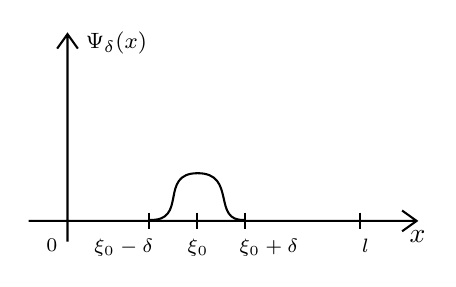
\begin{tikzpicture}[x=0.75pt,y=0.75pt,yscale=-1,xscale=1]
	%uncomment if require: \path (0,142); %set diagram left start at 0, and has height of 142
	
	%Shape: Axis 2D [id:dp28568967834010284] 
	\draw  (57,105) -- (243.89,105)(75.69,15) -- (75.69,115) (236.89,100) -- (243.89,105) -- (236.89,110) (70.69,22) -- (75.69,15) -- (80.69,22)  ;
	%Straight Lines [id:da6958476943035268] 
	\draw    (92,105) -- (180,105) (115,101) -- (115,109)(138,101) -- (138,109)(161,101) -- (161,109) ;
	%Curve Lines [id:da1534865928324396] 
	\draw    (115,104.5) .. controls (134,105.5) and (119.4,82.01) .. (138.4,82.01) .. controls (157.4,82.01) and (145,105.5) .. (161,104.5) ;
	%Straight Lines [id:da3525088238185259] 
	\draw    (75.69,105) -- (223.89,105) (216.69,101) -- (216.69,109) ;
	
	% Text Node
	\draw (239,108.4) node [anchor=north west][inner sep=0.75pt]    {$x$};
	% Text Node
	\draw (87,112.4) node [anchor=north west][inner sep=0.75pt]  [font=\scriptsize]  {$\xi _{0} -\delta $};
	% Text Node
	\draw (157,112.4) node [anchor=north west][inner sep=0.75pt]  [font=\scriptsize]  {$\xi _{0} +\delta $};
	% Text Node
	\draw (132,112.4) node [anchor=north west][inner sep=0.75pt]  [font=\scriptsize]  {$\xi _{0}$};
	% Text Node
	\draw (83,12.4) node [anchor=north west][inner sep=0.75pt]  [font=\footnotesize]  {$\Psi _{\delta }( x)$};
	% Text Node
	\draw (64,112.4) node [anchor=north west][inner sep=0.75pt]  [font=\scriptsize]  {$0$};
	% Text Node
	\draw (216,112.4) node [anchor=north west][inner sep=0.75pt]  [font=\scriptsize]  {$l$};
	
	
\end{tikzpicture}\vspace*{0.2cm}

\noindent При таком выборе $\Psi_{\delta}(x)$
\begin{equation}\label{l12:eq:4.1}
	\rho=\int\limits_{\xi_0-\delta}^{\xi_0+\delta}\rho\cdot\Psi_\delta(\xi)\,d\xi\quad\Longrightarrow\quad\int\limits_{\xi_0-\delta}^{\xi_0+\delta}\Psi_\delta(\xi)\,d\xi=1,\quad\forall\delta>0.
\end{equation}

Рассмотрим теперь задачу о свободных колебаниях струны с закреплёнными концами при
\begin{equation*}
	u(x,0)=0,\quad u_t(x,0)=\Psi_\delta(x).
\end{equation*}
Решение этой задачи обозначим через $u_\delta(x,t)$ и докажем, что $G(x,\xi_0,t)$ есть предел при $\delta\to0$ в смысле сходимости в среднем по $x$ на $[0,l]$ решений $u_\delta(x,t)$ при любом фиксированном $t$.
\begin{proof}
	В силу~\eqref{l12:eq:21} с учётом~\eqref{l12:eq:4.1}
	\begin{multline*}
		u_\delta(x,t)=\int\limits_0^l G(x,\xi,t)\cdot\Psi_\delta(\xi)\,d\xi=\int\limits_0^l\sum\limits_{k=1}^{\infty}\dfrac{\sin(\omega_k\cdot t)\cdot X_k(x)\cdot X_k(\xi)}{\omega_k}\cdot\Psi_\delta(\xi)\,d\xi=\\
		=\sum\limits_{k=1}^{\infty}\dfrac{\sin(\omega_k\cdot t)\cdot X_k(x)}{\omega_k}\cdot\int\limits_0^l X_k(\xi)\cdot\Psi_\delta(\xi)\,d\xi=\left|\parbox{0.12\textwidth}{\centering по теореме о среднем}\right|=\\=\sum\limits_{k=1}^{\infty}\dfrac{\sin(\omega_k\cdot t)}{\omega_k}\cdot X_k(x)\cdot X_k(\xi_{k\delta})\cdot\int\limits_{\xi_0-\delta}^{\xi_0+\delta}\Psi_{\delta}(\xi)\,d\xi=\sum\limits_{k=1}^{\infty}\dfrac{\sin(\omega_k\cdot t)}{\omega_k}\cdot X_k(x)\cdot X_k(\xi_{k\delta}),
	\end{multline*} 
	где $\xi_{k\delta}$ --- некоторая точка из интервала $(\xi_0-\delta,\xi_0+\delta)$.
	
	Положим $b_{k\delta}=\sin(\omega_k\cdot t)\cdot\big(X_k(\xi)-X_k(\xi_{k\delta})\big)$. Тогда, очевидно
	\begin{equation}\label{l12:eq:4.2}
		A_\delta\eqdef G(x,\xi,t)-u_\delta(x,t)=\sum\limits_{k=1}^{\infty}\dfrac{b_{k\delta}}{\omega_k}\cdot X_k(x).
	\end{equation}
	Пусть
	\begin{equation*}
		\widetilde{S}_n(x,t)\eqdef\sum\limits_{k=1}^{n}\dfrac{b_{k\delta}}{\omega_k}\cdot X_k(x).
	\end{equation*}
	Действуя также, как в конце пункта~\ref{lecture12section3} текущей лекции, можно показать, что последовательность $\widetilde{S}_n(x,t)$ фундаментальна в смысле сходимости в среднем по $x$ на $[0,l]$, при этом мы используем оценки $\omega_k\geqslant\alpha_0\cdot k$, $\alpha_0>0$ и $\displaystyle |b_{k\delta}|\leqslant2\cdot\sqrt{\frac{2}{l}}$. Следовательно, $\displaystyle\lim\limits_{n\to\infty}\widetilde{S}_n(x,t)$ существует при $\forall t$. Но $\widetilde{S}_n(x,t)$ --- последовательность частных сумм ряда~\eqref{l12:eq:4.2} и поэтому 
	\begin{equation*}
		\norm{A_{\delta}(x,t)-\widetilde{S}_n(x,t)}\to0,\quad\text{при }n\to\infty.
	\end{equation*}
	Отсюда в силу неравенства треугольника 
	\begin{equation*}
		\bigg|\norm{A_{\delta}(x,t)\vphantom{\widetilde{S}_n(x,t)}}-\norm{\widetilde{S}_n(x,t)}\bigg|\to0,\quad\text{при }n\to\infty.
	\end{equation*}
	Следовательно
	\begin{equation}\label{l12:eq:4.3}
		\norm{A_{\delta}(x,t)\vphantom{\widetilde{S}_n(x,t)}}^2=\lim\limits_{n\to\infty}\norm{\widetilde{S}_n(x,t)}^2=\sum\limits_{k=1}^{\infty}\dfrac{b_{k\delta}^2}{\omega_k^2}.
	\end{equation}
	Теперь по $\forall\eps>0$ $\exists N(\eps)\gg1$ так, что
	\begin{equation}\label{l12:eq:4.4}
		\sum\limits_{k=N+1}^{\infty}\dfrac{b_{k\delta}^2}{\omega_k^2}\leqslant\frac{\eps}{2},\quad\forall\delta,t.
	\end{equation}
	Далее при выбранном $N$ укажем $\delta_0>0$ столь малым, что при $\delta\leqslant\delta_0$
	\begin{equation}\label{l12:eq:4.5}
		b_{k\delta}^2\leqslant\dfrac{\omega_k^2\cdot\eps}{2\cdot N},\quad k=\overline{1,N}.
	\end{equation}
	Это можно сделать, так как $X_k(\xi)\in\Cfn[{[0,l]}]{}$ и $|\xi_0-\xi_{k\delta}|<\delta\leqslant\delta_0$. В силу~\eqref{l12:eq:4.5}
	\begin{equation}\label{l12:eq:4.6}
		\sum\limits_{k=1}^{N}\dfrac{b_{k\delta}^2}{\omega_k^2}\leqslant\dfrac{\eps}{2}.
	\end{equation}
	Из~\eqref{l12:eq:4.3},~\eqref{l12:eq:4.4} и~\eqref{l12:eq:4.6} вытекает, что 
	\begin{equation*}
		\norm{A_\delta(x,t)}^2\leqslant\eps\quad\text{при }\delta\leqslant\delta_0,\ \forall G.
	\end{equation*}
	Так как $\eps>0$ --- любое число, то тем самым доказано, что
	\begin{equation*}
		\lim\limits_{\delta\to0}\norm{G(x,\xi_0,t)-u_\delta(x,t)}=0.
	\end{equation*}
\end{proof}
\section[Свободные колебания однородной струны с другими г. у.]{Свободные колебания однородной струны с другими граничными условиями.}
\label{lecture12section5}
Мы рассмотрели подробно решение задачи~\eqref{l12:eq:10},~\eqref{l12:eq:11} с граничными условиями~\eqref{l12:eq:12}, то есть колебания струны с закреплёнными концами. Совершенно аналогично решается задача~\eqref{l12:eq:10},~\eqref{l12:eq:11} при других однородных граничных условиях на одном или обоих концах. Укажем все возможные варианты.
\vspace{0,4cm}

\noindent\underline{Левый конец}:\\[4pt]
$u(0,t)=0$ (закрепление), $u_x(0,t)=0$ (свободный конец), $u_x(0,t)=\sigma\cdot u(0,t)$, $\sigma>0$ (упругое закрепление).
\vspace{0,2cm}

\noindent\underline{Правый конец}:\\[4pt]  
$u(l,t)=0$ (закрепление), $u_x(l,t)=0$ (свободный конец), $u_x(l,t)=-\sigma\cdot u(l,t)$, $\sigma>0$ (упругое закрепление).
\vspace{0,4cm}

Таким образом, имеется всего девять ситуаций, одна из которых разобрана. Для каждой из не рассмотренных ситуаций надо пройти тот же путь, который мы прошли для задачи~\eqref{l12:eq:10}--\eqref{l12:eq:12}. Разница будет лишь в том, что найдутся (может приближённо) другие собственные значения $\lambda_k$  (то есть будет другая величина $\omega_k$) и другие собственные функции.
\vspace{0,2cm}

\noindent\textbf{Задание. }Решите задачи о свободных колебаниях однородной струны с любыми граничными условиями из названных выше.